\chapter{Tecnologias de Desenvolvimento}

\section{Docker}

O Docker é um sistema de virtualização que se baseia no empacotamento e uso de ambientes em \textit{containers}. O Docker diferente de outros sistemas de virtualização não necessita de Hardware virtualizado e nem necessariamente de uma instalação completa de um S.O. dentro do \textit{container} \cite{7742298}. Para seu funcionamento ele usa algumas \textit{features} do \textit{kernel} como o Cgroups e o namespaces, essas features são utilizadas para poder rodar os processos independentemente. Este modelo permite uma melhor organização da infraestrutura e, em simultâneo, mantém os ambiente seguros já que eles são separados. A Figura 4 compara a execução de imagens em um Linux Container e em Docker.

\begin{figure}[!htb]
     \centering
     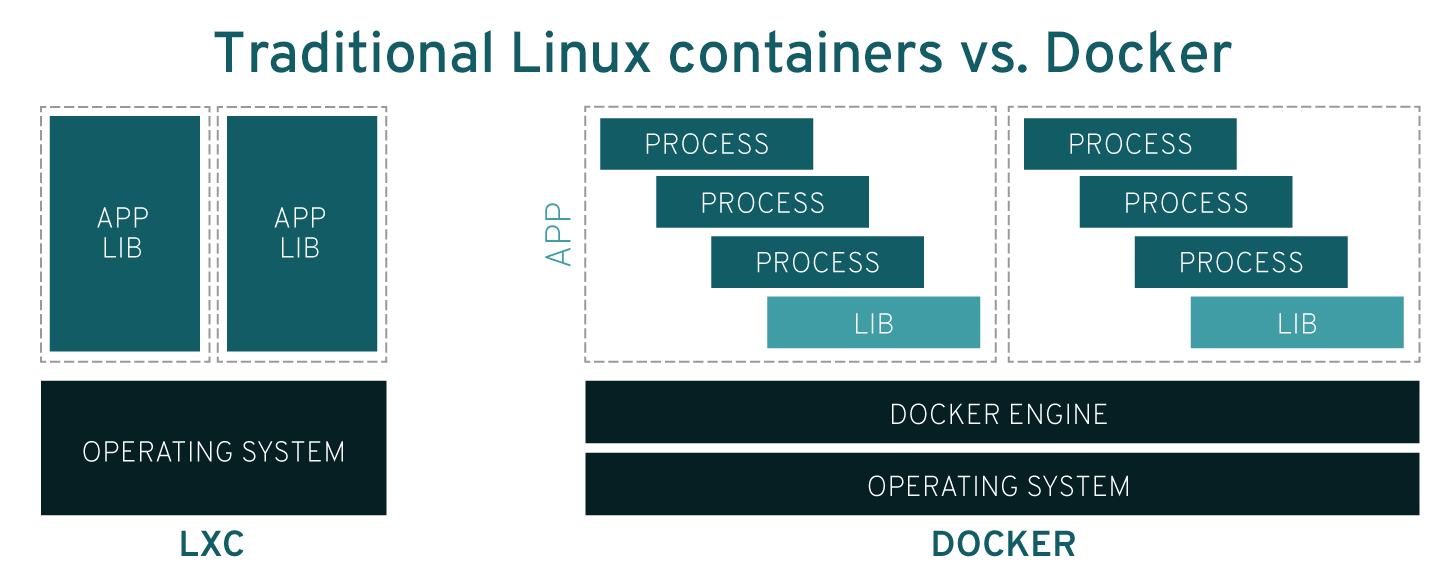
\includegraphics[width=15cm]{traditional-linux-containers-vs-docker_0.png}
     \caption{Figura do site RedHat sobre containers em Linux vs Docker~\cite{docker}}
     \label{Label de referência para a imagem}
\end{figure}

\section{Tecnologias de aplicação}

Além do Docker teremos algumas tecnologias que serão utilizadas no desenvolvimento do ambiente proposto.

\subsection{NodeJS}

Na aplicação de back-end a tecnologia de desenvolvimento será o NodeJS que é um \textit{runtime} de JavaScript que funciona em forma de execução assíncrona, permitindo a execução de código sem a necessidade de esperar o retorno de requisições \cite{7960064}. O Node foi criado pensando também em aplicações web escaláveis, sendo uma plataforma open-source multi-paradigmas.

\subsection{React}

O React é uma biblioteca do JavaScript que serve para a criação de interfaces de usuário. O React trabalha pensando em reaproveitamento de código criando componentes e pensando numa maior facilidade para descrição de estados e de conexão entre o CSS, JavaScript e HTML \cite{url:react}.

\subsection{SQLite}

O SQLite é um banco de dados relacional open-source prático e acessível que consegue atuar como o próprio servidor, já que ele insere seus dados dentro de si mesmo para funcionar. O nível de segurança desse banco não é tão alto, mas justamente isso também permite explorar outras vulnerabilidades dentro do ambiente \cite{5231398}.

\section{Ambiente local}

A imagem Docker estará disponível no repositório, após o download basta a execução que através do Dockerfile fará o ambiente ser configurado para permanecer sendo executado apenas de forma local, não permitindo que as aplicações sejam visualizadas pelo mundo exterior. Assim não haverá problemas com tráfego mal-intencionado na rede.